\section{Versuchsaufbau/-durchführung}
Eine schematische Darstellung des Aufbaus zur Aktivierung der verwendeten Proben befindet sich in Abbildung \ref{fig: neutronenquelle}.
\textbf{Hier noch ergänzen}
\begin{figure}
  \centering
  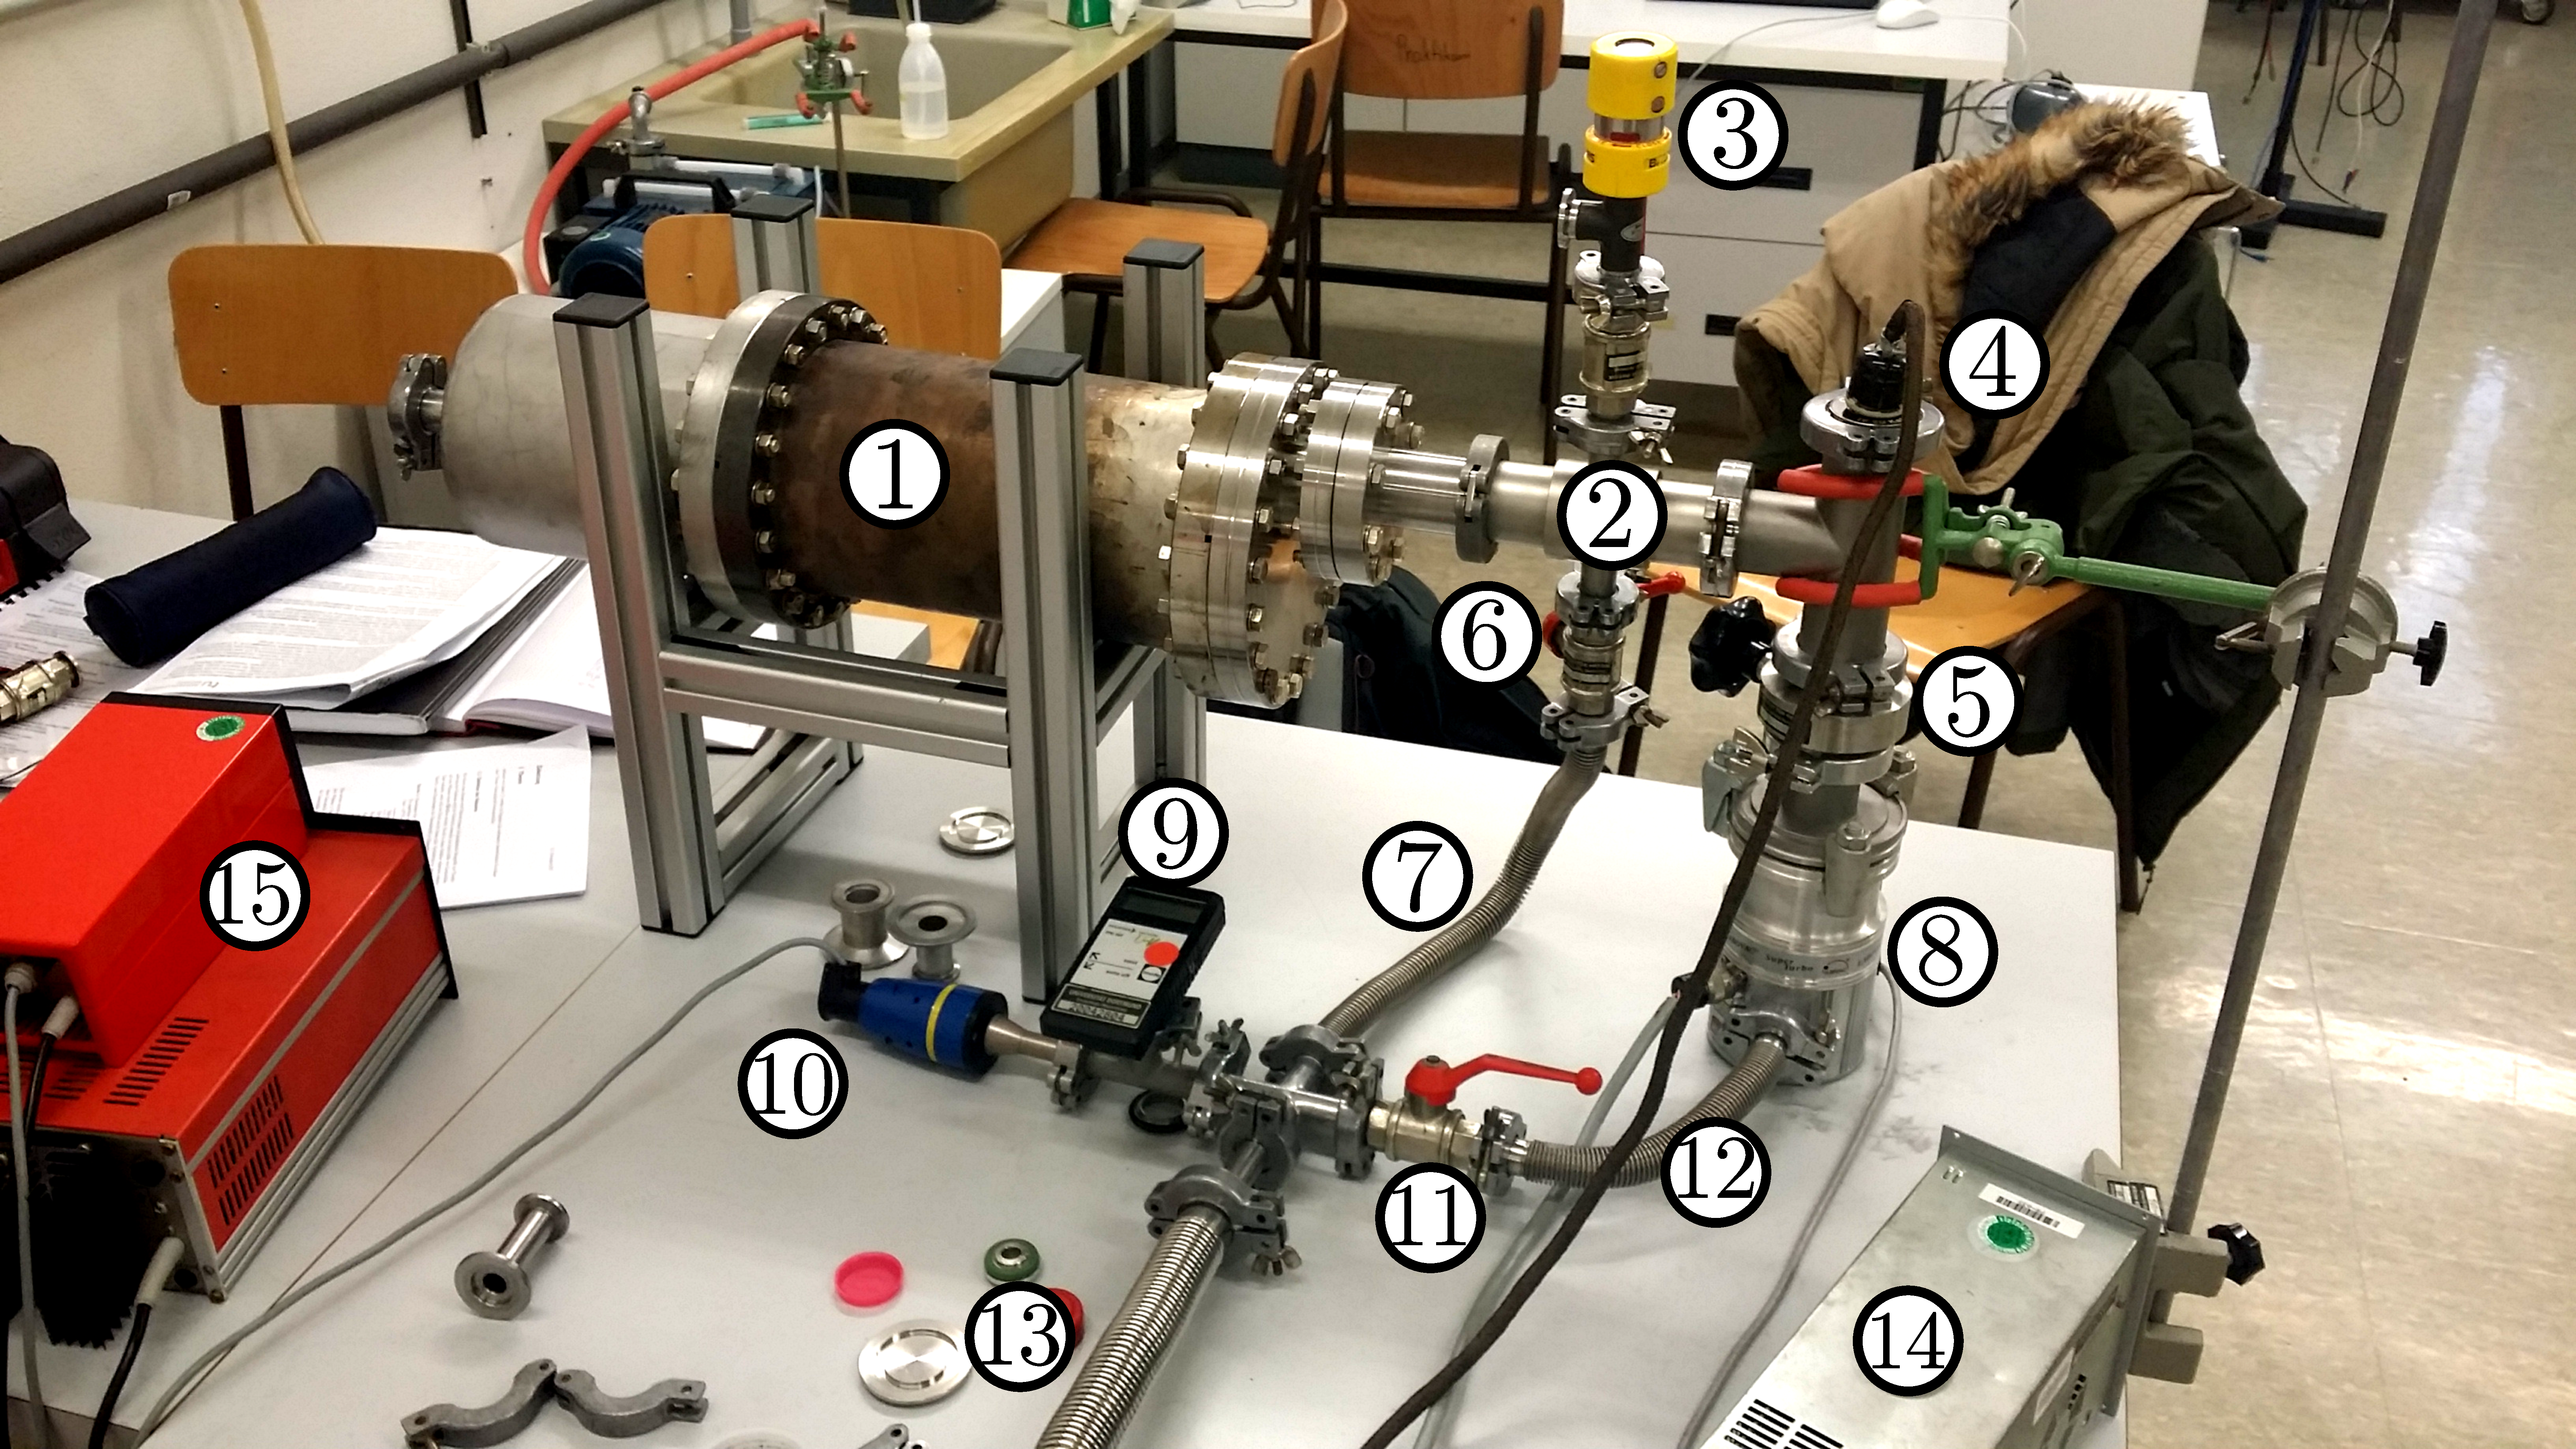
\includegraphics[width=0.5\textwidth]{pics/aufbau.png}
  \caption{Schematische Darstellung der Neutronenquelle \cite{anleitung702}.}
  \label{fig: neutronenquelle}
  \end{figure}

Im Anschluss an die Aktivierung der verwendeten Proben werden diese in den Aufbau nach Abbildung x integriert.

\begin{figure}
\centering
\includegraphics[width=0.5\textwidth]{pics/aufbau_2.png}
\caption{Aufbau zur experimentellen Bestimmung der Halbwertszeit \cite{anleitung702}.}
\label{fig: aufbau}
\end{figure}
